\documentclass[12pt,a4paper, xcolor=table]{article}
\usepackage{graphicx}
\usepackage[utf8]{inputenc}
\usepackage{eurosym}
\usepackage[spanish,es-tabla]{babel}
\usepackage[left=2cm, right=2cm, top=2cm, bottom=2cm]{geometry}
\usepackage{afterpage}
\PassOptionsToPackage{hyphens}{url}\usepackage{hyperref}
\usepackage{subfig}
\usepackage[table,xcdraw]{xcolor}

\usepackage{imakeidx}
\newcommand\blankpage{%
    \null
    \thispagestyle{empty}%
    \addtocounter{page}{-1}%
    \newpage}
\renewcommand*\contentsname{Índice: }

\makeindex
\let\olditemize\itemize
\def\itemize{\olditemize\itemsep=0pt}

\begin{document}
\setlength{\parindent}{0pt}
\begin{titlepage}
        \centering
        
\includegraphics[width=0.75\textwidth]{img/logo_uc3m.jpg}\par\vspace{2cm}
        {\huge\bfseries Práctica 2 \\ Análisis de las reseñas de Tripadvisor\par}
        \vspace{0.5cm}
        {\scshape\Large Inteligencia Artificial en las Organizaciones\par}
        \vspace{1.5cm}
        {\scshape\Large Grupo 83-1\par}
        \vspace{1.5cm}
        {\Large\itshape Miguel Gutiérrez Pérez\par}
        {\Large 100383537@alumnos.uc3m.es \par}
        \vspace{1cm}
        {\Large\itshape Mario Lozano Cortés\par}
        {\Large 100383511@alumnos.uc3m.es\par}
        \vspace{1cm}
        {\Large\itshape Alba Reinders Sánchez\par}
        {\Large 100383444@alumnos.uc3m.es\par}
        \vspace{1cm}
        {\Large\itshape Alejandro Valverde Mahou\par}
        {\Large 100383383@alumnos.uc3m.es\par}
        \vspace{5mm}
        {\large GitHub: \textbf{\textit{\href{https://github.com/Pheithar/InteligenciaArtificialOrganizaciones}{InteligenciaArtificialOrganizaciones}}}}
        \vfill

% Bottom of the page
        {\large \today\par}
\end{titlepage}

\tableofcontents

\newpage

\section{Introducción}

    La \textbf{Minería de Texto} es una técnica de minería de datos que busca extraer información útil y relevante de documentos de texto de diferentes fuentes diferentes, como puede ser páginas web, correos electrónicos, periódicos o redes sociales. Para ello se hace una identificación de patrones en los datos, como puede ser la repetición de palabras o conjuntos de palabras, estructuras sintácticas que se repiton a lo largo de los datos, etc.

    \vspace{3mm}

    Esta minería de texto tiene numerosas aplicaciones, y en esta práctica se van a desarrollar una clasificación en función a unas categorías predefinidas y un agrupamiento sin tener en cuenta estas categorías.

    \vspace{2mm}

    La colección de textos que se va a usar en la práctica consiste en un conjunto de reseñas de la página web \textit{Tripadvisor}, donde cada una tiene una clasificación de 1 a 5 estrellas.

    \begin{figure}[!h]
      \centering
      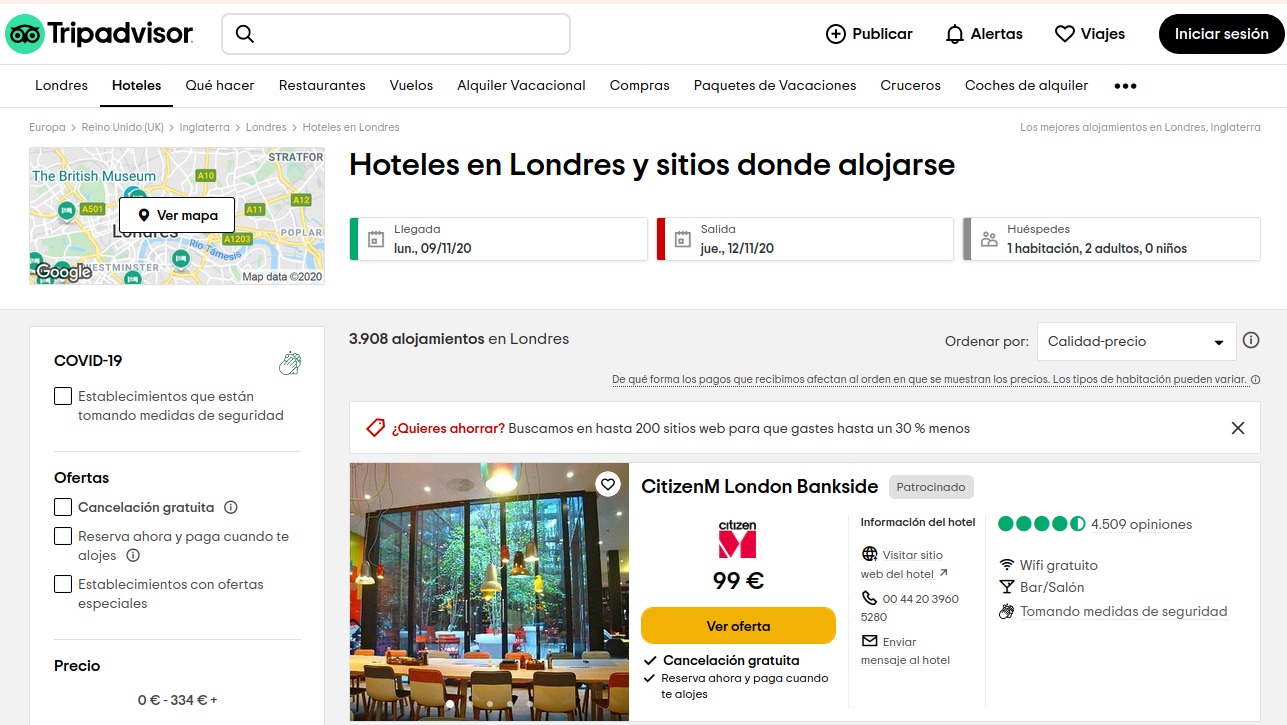
\includegraphics[width=14cm]{img/tripadvisor-main.png}
      \caption{Página de búsqueda de Tripadvisor}
    \end{figure}

    Las reseñas están en inglés, y en texto en plano, por lo tanto, para poder ser tratadas, tendrán que pasar por un proceso de preparación de datos.

    \begin{figure}[!h]
      \centering
      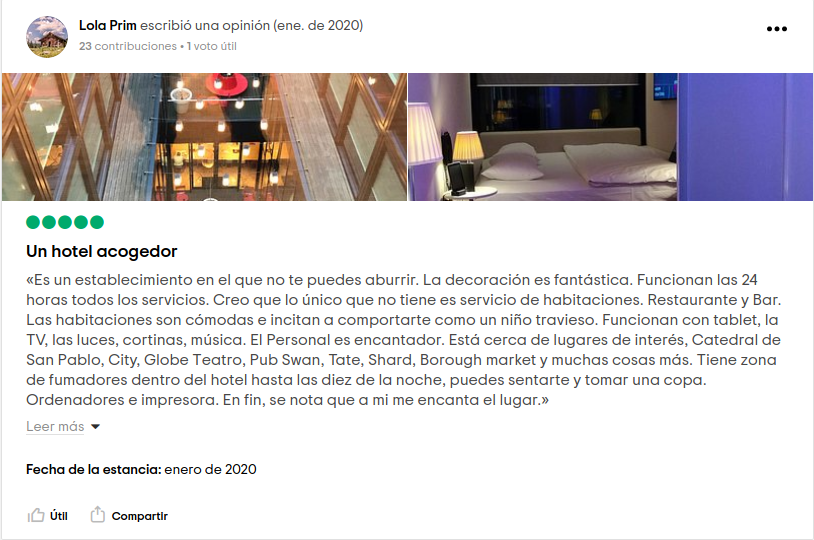
\includegraphics[width=10cm]{img/tripadvisor-review.png}
      \caption{Ejemplode reseña de Tripadvisor en \textit{español}}
    \end{figure}

    En la práctica se plantean dos problemas, uno de \textbf{aprendizaje supervisado} (clasificación), donde el objetivo es determinar la puntuación que le da un usuario a un hotel, en base a lo que escribe en su reseña; y otro de \textbf{aprendizaje no supervisado} (agrupamiento), cuyo objetivo es agrupar las diferentes reseñas en función a su contenido, sin tener en cuenta su puntuación.

    \vspace{3mm}


\section{Parte 1: Clasificación}
    \subsection{Análisis y preprocesado de datos}
        El primer paso que debe ser abordado en el desarrollo de esta práctica es el del procesado de los datos con el objetivo de \textbf{posibilitar la aplicación de minería de texto} gracias a la herramienta \textit{Weka}. Los datos sin tratar se encuentran contenidos en un archivo de formato \textit{csv} donde la primera columna se corresponde de con las reseñas en formato de texto y la segunda con el número de estrellas (valoración del 1 al 5) correspondientes a dicha reseña. De esta manera, la secuencia de operaciones lógicas a seguir para posibilitar el análisis con la herramienta propuesta son:

        \begin{itemize}
        \item Transformación del fichero desde el formato \textbf{\textit{csv}} al formato \textbf{\textit{arff}}
        \item Procesamiento propio de las técnicas de minería de texto en la herramienta \textit{Weka}
        \end{itemize}

        \subsubsection{De .csv a .arff}

          Como se ha comentado anteriormente el material proporcionado consta de un archivo en formato \textit{csv}. La mejor manera de convertirlo al formato \textit{arff} utilizado por \textit{Weka} es generar una estructura de directorios en función de la clasificación de la reseña para una vez dentro de cada uno de los directorios, encontrar un fichero por cada una de las reseñas. Dicha estructura se puede generar gracias a la herramienta de Macros contenida dentro del programa \textit{Excel}. Cabe destacar que esta estructura es óptima para el propósito seguido puesto que se proporciona un comando que en la opción \textit{CLI} de \textit{Weka} produce directamente un fichero \textit{arff} a partir de la estructura descrita.

        \subsubsection{Procesamiento específico de minería de texto}
          Una vez dentro de la herramienta \textit{Weka} se deben considerar técnicas de procesamiento específicas de la minería de texto, concretamente el filtro no supervisado \textbf{\textit{StringToWordVector}}, el cual permite convertir atributos basados en cadenas de caracteres en un conjunto numérico que representa la ocurrencia de las distintas palabras contenidas en el archivo seleccionado. Este filtro contiene \textbf{multitud de parámetros interesantes }que merece la pena reseñar de cara a la experimentación que se llevará a cabo para obtener el mejor modelo posible.

          \begin{itemize}
          \item \textbf{StopWords}: Formadas por palabras sin significado, es decir, aquellas que \textbf{no aportan información útil} al proceso de minería de texto que se pretende realizar. Se aporta una lista para la realización de la práctica, sin embargo \textbf{es importante reseñar que se añaden algunas más a ella para mejorar los resultados del análisis}. Algunas de las palabras añadidas incluyen números y palabras sin sentido consecuencia posiblemente de faltas de ortografía a la hora de escribir las reseñas.

          \item \textbf{TFTransform}: Establece si la frecuencia de las palabras debe transformarse a $log(1+f_{ij})$ siendo $f_{ij}$ la frecuencia de la palabra i en el documento j.
          \item \textbf{IDFTransform}: Establece su la frecuencia de palabras en un documento debe trasnformarse a $f_{ij} * log(\frac{numeroDocumentos}{numeroDocumentos\_con\_i})$ siendo $f_{ij}$ la frecuencia de la palabra i en el documento j.
          \item \textbf{outputWordCounts}: Número exacto de ocurrencias de una palabra en vez de indicar únicamente presencia.
          \item \textbf{stemmer}: Algoritmo de \textit{stemming} a usar. Conviene recordar que un algoritmo de \textit{stemming} trata de reducir las palabras a sus raíces.
          \item \textbf{normalizeDocLength}: Establece si se normalizan las frecuencias de palabras de un documento.
          \item \textbf{minTermFreq}: Determina el número mínimo de ocurrencias que debe tener una palabra para se tenida en cuenta.
          \item \textbf{tokenizer}: Algoritmo de \textit{tokenizing} que se aplica. Conviene recordar que un algoritmo de \textit{tokeninzing} divide una secuencia de caracteres en tokens que pueden ser desde palabras a frases completas.

          \end{itemize}

      \subsection{Experimentación}
        Para realizar los experimentos, se han realizado combinaciones de los distintos opciones que habilita la herramienta de \textit{Weka} con el filtro \textit{StringToWordVector}, para buscar la combinación que permita obtener los mejores resultados para este conjunto de datos. Este filtro, tal y como su nombre indica, transforma un atributo compuesto por texto, en un conjunto de atributos que representa la información de ese texto.

      \subsubsection{Experimentación básica}
        Los primeros experimentos que se han realizado consisten en modifcar exclusivamente una opción del filtro en cada uno de los experimentos, para comprobar cuales son los que generan los mejores resultados por separado. Los experimentos realizados son los siguientes:

        \begin{itemize}
          \item \textbf{Experimento 0}: Es el experimento base, respecto al que se van a comparar el resto.
          \item \textbf{Experimento 1}: En este experimento se prueba las combinaciones que se pueden hacer entre la opción \textit{IDFTransform} y \textit{TFTransform}, por lo que está compuesto de 3 subexperimentos.
          \begin{itemize}
            \item \textbf{Experimento 1-1}: \textit{IDFTransform} \textbf{True} y \textit{TFTransform} \textbf{False}.
            \item \textbf{Experimento 1-2}: \textit{IDFTransform} \textbf{False} y \textit{TFTransform} \textbf{True}.
            \item \textbf{Experimento 1-3}: \textit{IDFTransform} \textbf{True} y \textit{TFTransform} \textbf{True}.
          \end{itemize}
          \item \textbf{Experimento 2}: Este experimento prueba a activar la opción \textit{outputWordCounts}
          \item \textbf{Experimento 3}: En este experimento se prueba el uso de diferentes \textit{stemmer}, con dos subexperimentos.
          \begin{itemize}
            \item \textbf{Experimento 3-1}:Usando el \textit{LovinsStemmer}
            \item \textbf{Experimento 3-2}:Usando el \textit{IterativeLovinsStemmer}
          \end{itemize}
          \item \textbf{Experimento 4}: En este experimento se prueba a cambiar el valor por defecto de la opción de \textit{minTermFreq}, que es 1. Tiene 7 subexperimentos.
          \begin{itemize}
            \item \textbf{Experimento 4-1}: El valor de \textit{minTermFreq} es 2
            \item \textbf{Experimento 4-2}: El valor de \textit{minTermFreq} es 5
            \item \textbf{Experimento 4-3}: El valor de \textit{minTermFreq} es 10
            \item \textbf{Experimento 4-4}: El valor de \textit{minTermFreq} es 25
            \item \textbf{Experimento 4-5}: El valor de \textit{minTermFreq} es 125
            \item \textbf{Experimento 4-6}: El valor de \textit{minTermFreq} es 250
            \item \textbf{Experimento 4-7}: El valor de \textit{minTermFreq} es 625
          \end{itemize}
          \item \textbf{Experimento 5}: Este experimento prueba la eficacia de la opción \textit{normalizeDocLength} sobre tod el conjunto de datos.

        \end{itemize}

        Para cada uno de los experimentos mostrados se deben ejecutar distintos algoritmos de clasificación con el objetivo de averiguar cuál de ellos funciona mejor dada la configuración elegida por el experimento. Los algoritmos de clasificación seleccionados por ser los más ampliamente extendidos son:
    
        \begin{itemize}
        \item J48
        \item Random Forest
        \item JRip
        \item IBk
        \item Naive Bayes
        \end{itemize}

        \begin{table}[h]
            \centering
            \begin{tabular}{|c|c|c|c|c|c|}
            \hline
            \rowcolor[HTML]{DAE8FC}
            \textbf{ID Experimento} & \textbf{J48} & \textbf{RandomForest} & \textbf{JRip} & \textbf{IBk} & \textbf{Naive Bayes} \\ \hline
            0                       & 38.88\%                   & 51.80\%        & 35.28\%                    & 26.12\%         & 49.76\%            \\ \hline
            1-1                     & 38.88\%                   & 52.64\%        & 33.32\%                    & 26.12\%         & 49.76\%            \\ \hline
            1-2                     & 38.88\%                   & 52.04\%        & 35.64\%                    & 26.12\%         & 49.76\%            \\ \hline
            1-3                     & 38.88\%                   & 51.84\%        & 33.76\%                    & 26.12\%         & 49.76\%            \\ \hline
            2                       & 44.92\%                   & 59.92\%        & 40.36\%                    & 27.76\%         & 49.28\%            \\ \hline
            3-1                     & 38.88\%                   & 51.56\%        & 34.92\%                    & 26.12\%         & 49.76\%            \\ \hline
            3-2                     & 38.44\%                   & 51.68\%        & 34.96\%                    & 26.36\%         & 49.76\%            \\ \hline
            4-1                     & 38.88\%                   & 51.56\%        & 33.32\%                    & 26.12\%         & 49.76\%            \\ \hline
            4-2                     & 38.88\%                   & 51.56\%        & 33.32\%                    & 26.12\%         & 49.76\%            \\ \hline
            4-3                     & 38.56\%                   & 52.32\%        & 34.16\%                    & 26.64\%         & 49.80\%            \\ \hline
            4-4                     & 39.16\%                   & 52.44\%        & 36.20\%                    & 28.72\%         & 50.32\%            \\ \hline
            4-5                     & 38.68\%                   & 49.16\%        & 34.96\%                    & 33.48\%         & 47.32\%            \\ \hline
            4-6                     & 34.64\%                   & 34.64\%        & 40.96\%                    & 32.48\%         & 40.44\%            \\ \hline
            4-7                     & 27.04\%                   & 27.04\%        & 25.80\%                    & 25.56\%         & 25.12\%            \\ \hline
            5                       & 39.20\%                   & 51.68\%        & 34.04\%                    & 20.00\%         & 48.8\%            \\ \hline
            \end{tabular}
            \caption{Experimentos realizados}
                \label{fig:graf_exp1}
        \end{table}

        La tabla 1 muestra la relación de experimentos realizados junto con los resultados en cada uno de los algoritmos de clasificación seleccionados. Un vistazo rápido a la misma permite averiguar que el algoritmo de clasificación más prometedor es \textbf{RandomForest}, por lo tanto a continuación se abre una nueva ventana en la experimentación, la cual tratará de afinar la configuración de los distintos parámetros propuestos en los experimentos para RandomForest.

        \subsubsection{Experimentación avanzada}

        Como en los experimnentos básicos se prueba que los mejores resultados son siempre obtenidos con el algoritmo de \textbf{RandomForest}, en esta experimentación avanzada, tan solo se va a evaluar con él.

        \vspace{3mm}

        La experimentación avanzada consiste en realizar combinaciones entre las opciones del filtro que generan mejores resultados en el apartado anterior, para intentar encontrar una transformación que maximice el resultado obtenido.

        \begin{itemize}
          \item \textbf{Experimento 6}: En este útimo experimento se analizan los resultados que se obtienen al cambiar la opciónd e \textit{tokenizer}. Tiene 2 subexperimentos.
          \begin{itemize}
            \item \textbf{Experimento 6-1}: Se utiliza el \textit{tokenizer} de \textit{NGramTokenizer}
            \item \textbf{Experimento 6-2}: Se utiliza el \textit{tokenizer} de \textit{AlphabeticTokenizer}
          \end{itemize}
          \item \textbf{Experimento 7}: Se prueba una combinación de \textit{IDFTransform}, \textit{TFTransform} y \textit{outputWordCounts}.
          \item \textbf{Experimento 8}: Se seleccionan las siguientes opciones: \textit{IDFTransform}, \textit{TFTransform}, \textit{outputWordCounts}, como \textit{tokenizer} el \textit{NGramTokenizer} y un valor de \textit{minTermFreq} de 25.
        \end{itemize}

        \begin{table}[h]
            \centering
            \begin{tabular}{|c|c|}
            \hline
            \rowcolor[HTML]{DAE8FC}
            \textbf{ID Experimento} & \textbf{RandomForest} \\ \hline
            6-1                     & 52.12\%               \\ \hline
            6-2                     & 51.40\%               \\ \hline
            7                       & 59.00\%               \\ \hline
            8                       & 60.28\%               \\ \hline
            \end{tabular}
            \caption{Experimentos avanzados}
                \label{fig:graf_exp1}
        \end{table}

        La tabla 2 muestra los resultados obtenidos en la experimentación avanzada, siendo el experimento 8 el que obtiene los mejores resultados. La siguiente sección trata de dar sentido a los resultados obtenidos.

    \subsection{Comentario de los resultados obtenidos}
    \textbf{ La sección experimentación básica permite descubrir qué algoritmo de clasificación tiene los mejores resultados} además de dar \textbf{indicaciones sobre qué configuración del filtro de minería de datos mejora} los mismos. Por lo tanto, la sección avanzada descubre cómo es posible mejorar el clasificador seleccionado a través de la afinación de parámetros del filtro, descubriendo, como era de esperar, que una combinación de los mejores parámetros del filtro permite añadir exactitud al clasificador sumando los efectos de las mejoras aplicadas. 
    
    \vspace{3mm}
    
    Así los resultados arrojados seleccionan al \textit{experimento 8} dado que \textbf{limita el ruido} en los datos incluyendo una\textbf{ frecuencia mínima de aparición} de términos, además, permite \textbf{aumentar la precisión} al establecer un algoritmo de \textit{tokeninzing} que unido al establecimiento de \textbf{métricas sobre la frecuencia y número de ocurrencias} de las palabras permite aumentar y mejorar la calidad de la información extraída de los datos, permitiendo así una generalización mayor, logrando de esta manera cumplir con el objetivo de clasificar las reseñas de \textit{Tripadvisor}.

\newpage

\section{Parte 2: Clustering}

En la segunda parte de esta práctica se va a realizar una aproximación mediante \textbf{\textit{clustering}}, pero antes de esto, recordar que esta técnica consiste en agrupar instancias sin etiquetar de manera que las instancias pertenecientes aun mismo grupo sean más similares entre sí que con las de otro grupo diferente. 

\vspace{2mm}

En este caso, se agruparán las instancias procesadas que obtuvieron un mejor resultado en la primera parte de la práctica, esta agrupación se hará con el algoritmo \textbf{\textit{K-Medias}}, que se basa en el valor medio de las distancia de cada grupo para generar los grupos. 

\vspace{1mm}

Este proceso se vuelve a realizar en \textit{Weka}, y se compone de los siguientes pasos:

\begin{itemize}
    \item Cargar el archivo \textit{.arff} con los datos generado en la parte anterior.
    \item Generar diferentes modelos a partir de estos datos con \textit{K-Medias} y compararlos.
    \item Analizar el mejor modelo obtenido.
    \item Ejecutar diversos algoritmos de generación de reglas y árboles de decisión con el mejor modelo obtenido.
\end{itemize}


\subsection{Experimentación}

Los experimentos que se llevan a cabo son los que se muestran en la en la Figura X. Los parámetros del algoritmo que se modifican son la \textit{seed} (10, 20 y 30), el \textit{números de clusters} (2, 3, 4, 5 y 6) y el \textit{tipo de distancia} (Euclidea y Manhattan).

\begin{figure}[h]
    \centering
    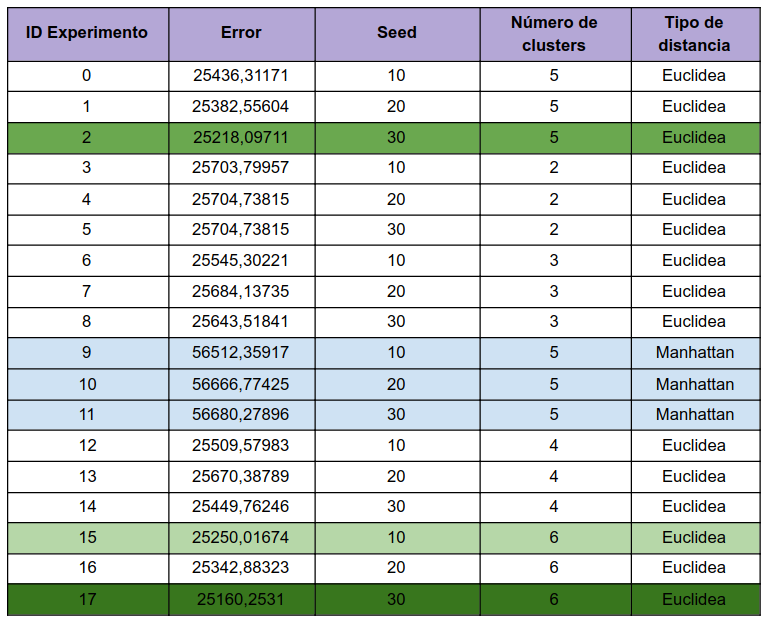
\includegraphics[width=400px]{img/experimentos.png}
    \caption{Tabla de experimentos con \textit{K-Medias}}
    \label{fig:graf_exp1}
\end{figure}


Como se puede apreciar en la Figura X, se prueba para un mismo número de clusters las 3 seeds. Cabe destacar que los experimentos probados con distancia de \textit{Manhattan} cometen mucho más error que los que usan la \textit{Euclidea}. Por este motivo en la gráfica donde se comparan los errores no se añaden, ya que no son relevantes.

\vspace{2mm}

Los errores cometidos por los experimentos que usan distancia \textit{Euclidea} varían en el rango de 25160.25, siendo este el mejor, a 25704.73, siendo este el peor. De estos, los mejores resultados son los marcados en verde.

\vspace{2mm}

Este error representa la suma de las distancias medias a cada cluster, por ello cuanto menor sea el error menor serán estas distancias y como consecuencia las instancias estarán mejor agrupadas.

\vspace{3mm}


A continuación se muestra en la Figura X la gráfica comparativa de los errores para poder visualizar mejor los errores de cada experimento.

\begin{figure}[h]
    \centering
    \includegraphics[width=400px]{img/Comparación errores.png}
    \caption{Gráfica comparativa de los errores}
    \label{fig:graf_exp1}
\end{figure}

Por lo tanto, se concluye con que el mejor resultado es el obtenido en el \textbf{Experimento 17}, así que en la siguiente sección se va a analizar en detalle este modelo.

\newpage


\subsection{Mejor modelo}

El mejor modelo es el obtenido con el Experimento 17, se compone de \textbf{6 clusters} aunque según la gráfica de la Figura X, parece que deja 2 clusters vacíos. Mientras que el cluster 4 es el que tiene mayor número de elementos seguido del cluster 5. Por otro lado los clusters 2 y 3 tienen muchos menos elementos.

\begin{figure}[h]
    \centering
    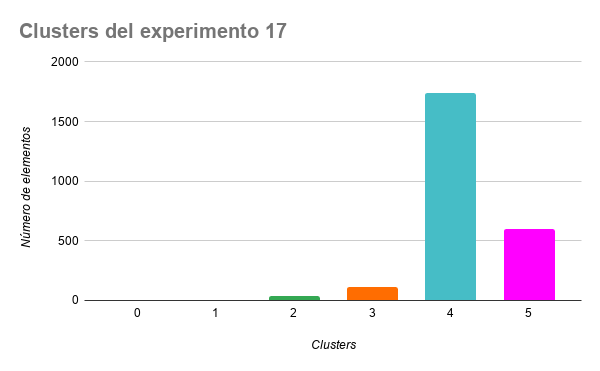
\includegraphics[width=300px]{img/clusters_del_experimento_17.png}
    \caption{Gráfica clusters Experimento 17}
    \label{fig:graf_exp1}
\end{figure}

Ya que con la Figura X no se puede afirmar que los clusters 0 y 1 estén vacíos, se van a visualizar los datos en la siguiente tabla de la Figura X.

\begin{figure}[h]
    \centering
    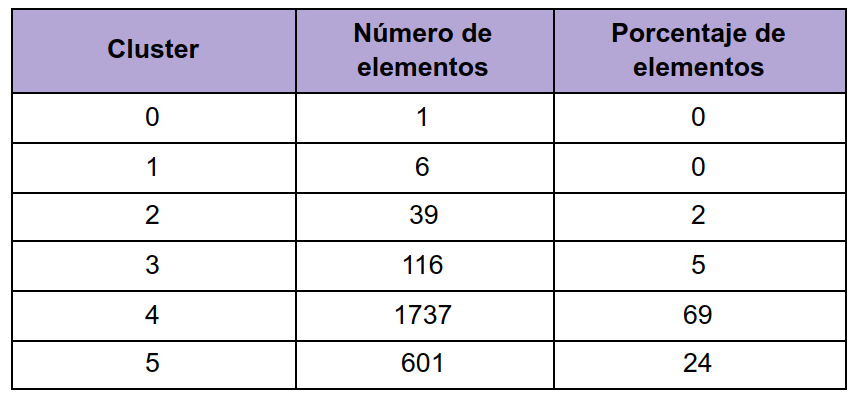
\includegraphics[width=300px]{img/clusters_mejor_exp.png}
    \caption{Tabla clusters Experimento 17}
    \label{fig:graf_exp1}
\end{figure}

\newpage

Una vez que se tienen los números concretos se observa que los cluster 0 y 1 no están vacíos pero poseen muy pocos elementos, 1 y 6 respectivamente. Por lo tanto, se llega a la conclusión de que estos elementos son \textit{outliers} y no aportan nada.

\vspace{4mm}

Tras este análisis del mejor modelo, se ejecutan los siguientes algoritmos de generación de reglas y árboles de decisión con este modelo para descibrir los clusters:

\begin{itemize}
    \item \textit{PART}
    \item \textit{J48}
    \item \textit{RandomForest}
    \item \textit{JRip}
\end{itemize}


\begin{figure}[h]
    \centering
    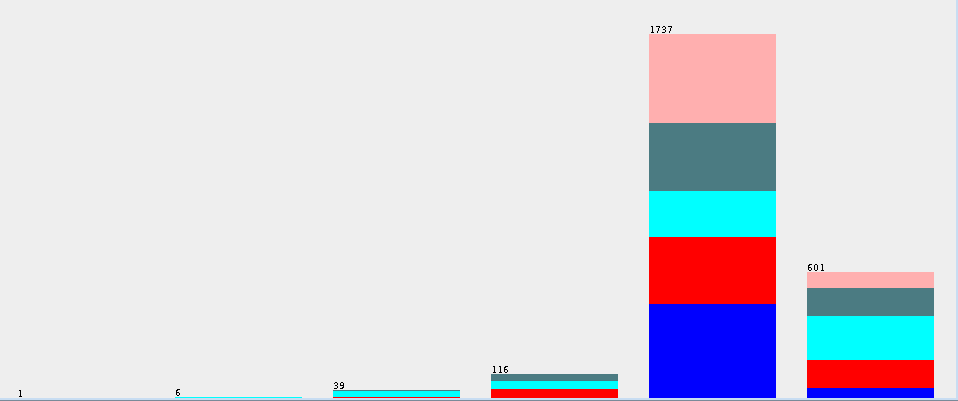
\includegraphics[width=300px]{img/clusters_class.png}
    \caption{Gráfica clusters-clase Experimento 17}
    \label{fig:graf_exp1}
\end{figure}





\section{Conclusiones}

\section{Contexto de la práctica}


\clearpage

\section{Referencias}
    \begin{itemize}
        \item [1.] Introduction to Neurons in Neural Networks. Medium. Consultado en Octubre 2020. Url: \\
        \href{https://medium.com/artificial-neural-networks/introduction-to-neurons-in-neural-networks-71828d040a65}{https://medium.com/artificial-neural-networks}
    \end{itemize}
\printindex



  \section{Anexos}
  \begin{itemize}
    \item [1.] Perceptron Multicapa usando '\textit{K Fold}'\\
    \textbf{\textit{perceptron\_kfold.py}}
    \item [2.] Perceptron Multicapa usando '\textit{split percentage}'\\
    \textbf{\textit{perceptron\_split.py}}
    \item [3.] Programa para realizar la predicción de los modelos\\
    \textbf{\textit{predict.py}}
    \item [4.] Tabla de resultados de los experimentos de la primera parte\\
    \textbf{\textit{valores\_reales\_vs\_predicciones\_\&\_errores\_absolutos\_parte1.xlsx}}
    \item [5.] Tabla de resultados de los experimentos de la segunda parte\\
    \textbf{\textit{valores\_reales\_vs\_predicciones\_\&\_errores\_absolutos\_parte2.xlsx}}
  \end{itemize}


\end{document}
